\documentclass[svgnames]{l3doc}
\usepackage{pdfpages, twemojis}
\usepackage[osf, mono = false]{libertine}
\usepackage[fontset = fandol, linespread = 1.2, autoindent = 0pt]{ctex}
\AddToHook{env/function/before}{\vspace*{-.5\baselineskip}}
\ExplSyntaxOn \makeatletter
\DeclareDocumentCommand \key { s m }
  {
    \IfBooleanTF {#1} { \textcolor{red}{\ttfamily \bfseries #2} }
      {
        \ttfamily
        \seq_set_from_clist:Nn \l_tmpa_seq {#2}
        \seq_set_map:NNn \l_tmpb_seq \l_tmpa_seq
          { \exp_not:n { \textcolor{red}{\bfseries ##1} } }
        \seq_use:Nn \l_tmpb_seq { ,~ } \:=\:
      }
  }
\DeclareCommandCopy \val \meta
\def \TFF {true\textup{\textbar\underline{\textbf{false}}}}
\def \TTF {\textup{\underline{\textbf{true}}\textbar}false}
\def \HoLogo@ApLaTeX #1{
  \HOLOGO@mbox {A\kern -.05em p\kern -.05em \hologo{LaTeX}}}
\makeatother \ExplSyntaxOff
\newlist{keyval}{itemize}{10}
\setlist[keyval]{leftmargin = 0pt, labelsep = 0pt}
\makeindex
\title{^^A
  \bfseries \cls{litetable} 宏包 --- 多彩的课程表\thanks{^^A
    \url{https://github.com/myhsia/litetable},
    \url{https://ctan.org/pkg/litetable}^^A
  }^^A
}
\author{^^A
  夏明宇 \texttt{<^^A
    \href{mailto:xiamingyu@westlake.edu.cn}{xiamingyu@westlake.edu.cn}>^^A
  }\thanks{^^A
    \href{https://github.com/ljguo1020}{郭李军}^^A
    开发了解析 \meta{left} \texttt{->} \meta{right} 型数据结构的接口.^^A
  }^^A
}
\date{Released 2025-08-20\quad \texttt{v3.7B}}

\begin{document}

\maketitle

\begin{documentation}

\section{介绍}

\pkg{litetable} 宏包提供了一个多彩的课程表设计,
基于 Ti\textit k\/Z
由 \pkg{expl3} 开发.
支持 \hologo{pdfLaTeX},\hologo{XeLaTeX},\hologo{ApLaTeX} 和
\hologo{LuaLaTeX} 等多种编译方式. 点击跳转
\href{http://mirrors.ctan.org/macros/latex/contrib/litetable/litetable.pdf}{[\textsf{English}]}
\href{http://mirrors.ctan.org/macros/latex/contrib/litetable/litetable-zh-hk.pdf}{[\textsf{繁体粤語}]} 手册.

\section{用户接口}

要加载此宏包,只需写下
\begin{quote}
  |\usepackage{litetable}|
\end{quote}

\DescribeEnv{litetable}
环境 \env{litetable} 可生成空白课程表,
需在命令 \cs{timelist} 和 \cs{weeklist} 后执行
\begin{quote}
  |\begin{litetable}|
    \oarg{keys} \marg{title} \oarg{keys}| ... |%
  |\end{litetable}|
\end{quote}
强制参数用于设定课程表标题,
可选参数接受以下键
\begin{keyval}
  \item [\key{scale}] \textcolor{gray}{\val{float} 可设置课程表的缩放比例(默认值: |1.0|).}
  \item [\key{color}] \val{color} 可设置课程表框架的背景色
  (默认值:|gray|),键名可省略.
  \item [\key{sem}] \val{string}
  可设置页面右上角的学期信息.
  \item [\key{hline}] \val{string} 可设置水平线的样式
  (默认值:|solid|).
\end{keyval}

\begin{function}{\weeklist}
  \begin{syntax}
    \cs{weeklist} \oarg{keys} \marg{list} \oarg{keys}
  \end{syntax}
  强制参数接收数组,
  用于设置课程表顶部的工作日列表和列宽.
  可选参数接受以下键
  \begin{keyval}
    \item [\key{format}] \val{format commands}
    可设置工作日列表格式(默认值:|\bfseries|).
    \item [\key{sep}] \val{string}
    可设置工作日列表的分隔符.
  \end{keyval}
  \begin{verbatim}
    \weeklist [ format = \bfseries \scshape, sep = \textbar ]
      { Mon -> 1.05, Tue -> 1.05, Wed -> 1.1, Thu -> 1.1, Fri -> .9 }
  \end{verbatim}
\end{function}

\begin{function}{\timelist}
  \begin{syntax}
    \cs{timelist} \oarg{keys} \marg{list} \oarg{keys}
  \end{syntax}
  强制参数均接收数组,用于设置课程表的左侧的时间列表.
  可选参数接受以下键
  \begin{keyval}
    \item [\key{numformat}] \val{format}
    可设置时间列表的序号字体
    (默认值:|\ttfamily \bfseries|).
    \item [\key{timeformat}] \val{format} 可设置时间列表的时间字体
    (默认值:|\ttfamily|).
    \item [\key{hidetime}] \val\TFF 用于隐藏时间列表中的时间,只保留序号.
    (初始值:|false|).
  \end{keyval}
  \begin{verbatim}
    \timelist [ numformat = \bfseries, timeformat = \ttfamily ]
      { 08:30 -> 10:00, 10:30 -> 12:00, 13:00 -> 14:30, 15:00 -> 16:30 }
  \end{verbatim}
\end{function}

\begin{function}{\course}
  \begin{syntax}
    \cs{course} \oarg{keys} \marg{start} \oarg{keys} \marg{end} \oarg{keys}
  \end{syntax}
  用于在当前工作日添加课程盒子,
  需在 \env{litetable} 环境中执行.
  两个强制参数分别用于设置课程的开始和结束序号.
  可选参数接收下列键
  \begin{keyval}
    \item [\key{color}] \val{color} 用于设置课程盒子的颜色
    (默认值:|teal|). 键名可省略.
    \item [\key{subject}] \val{string} 用于设置课程名称.
    \item [\key{location}] \val{string} 用于设置课程地点.
    \item [\key{lecture}] \val{string} 用于设置授课教师.
    \item [\key{comment}] \val{string} 用于给课程添加脚注.
  \end{keyval}
  \begin{texnote}
    \begin{itemize}[leftmargin = 2em]
      \item 若 \meta{start} |=| \meta{end}(课程盒子的高度为 $1$),
      则 \key*{location} 和 \key*{lecture} 将输出在同一行,
      并且 \key*{comment} 将隐藏.
      \item 即使误将 \meta{start} 和 \meta{end} 写反,
      模板也会自动纠正.
      \item 若 \key*{location} 和 \key*{lecture} 均未使用,
      则 \key*{subject} 将输出在课程盒子的
      竖直方向中心.
      \item 超出课程表范围的课程盒子将不显示,
      并会返回警告.
      输入用例见 Appendix \ref{mwe}.
    \end{itemize}
  \end{texnote}
\end{function}

\begin{function}{\newday}
  \begin{syntax}
    \cs{newday} \oarg{integral value}
  \end{syntax}
  使其后面添加的课程盒子后移 \meta{intergal value} 个工作日.
  可选参数的默认值为 |1|.
\end{function}

\begin{function}{\more}
  \begin{syntax}
    \cs{more} \marg{comment}
  \end{syntax}
  在课程表的右下角添加备注.
\end{function}

\clearpage \appendix \linespread{1.25}

\section{工作示例} \label{mwe}

\verbatiminput{litetable-demo.tex}

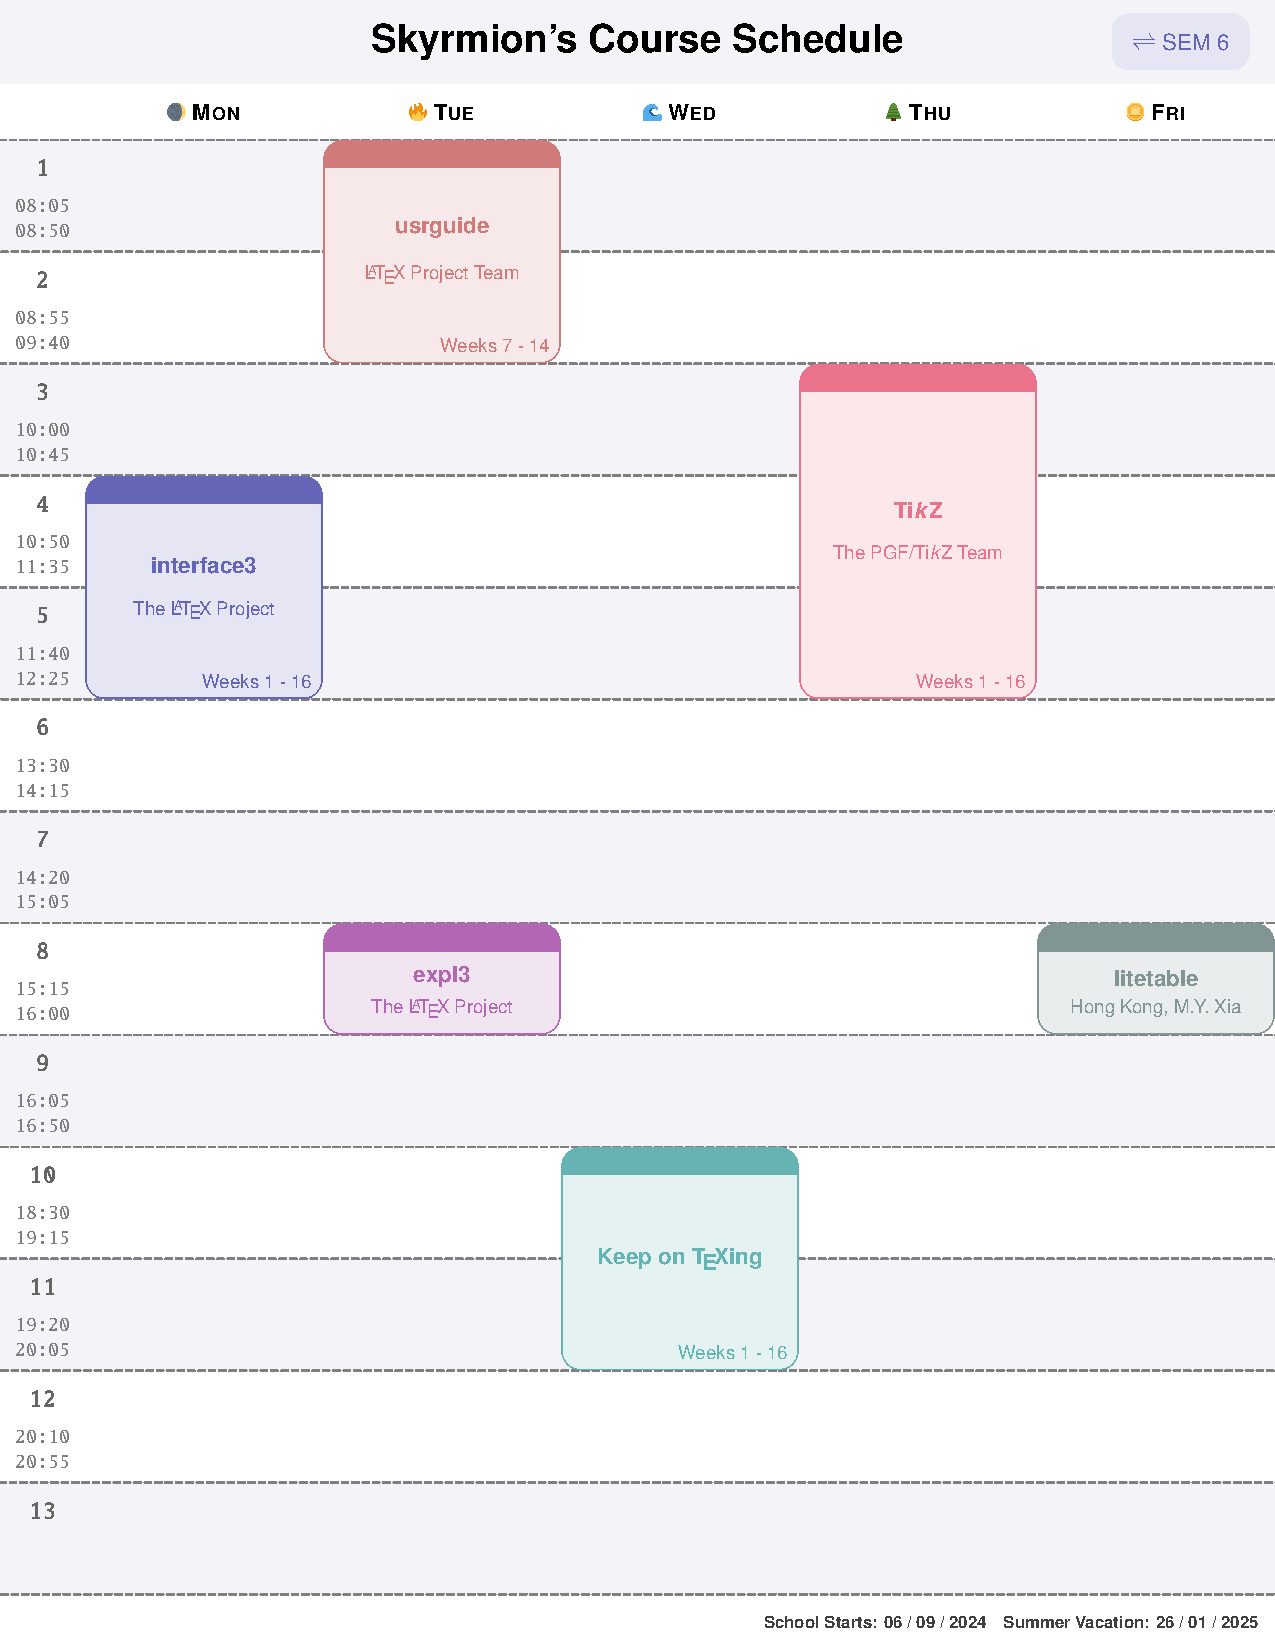
\includepdf{litetable-demo.pdf}

\end{documentation}

\IndexPrologue{%
  \part*{索引}
  \markboth{索引}{索引}
  \addcontentsline{toc}{part}{索引}
  意大利体的数字表示描述对应索引项的页码;
  带下划线的数字表示定义对应索引项的代码行号;
  罗马字体的数字表示使用对应索引项的代码行号.
}

\PrintIndex

\end{document}
